\section{Overlapping and accurate representations}
\label{section:overlapping-experiment}

The goal of the next experiment is to identify the required conditions for maintaining the matching representations of in-distribution samples, i.e., overlapping histograms for training and testing data presented in previous sections (e.g., figures \ref{fig:hists-md-samples}, \ref{fig:hists-knn-samples} and \ref{fig:hists-dimensions}). The research is conducted, considering primarily the dimensions of feature vectors $d$ and the number of samples $n$.

\vspace{2.0em}  % NOTE: Just to expand the elements on page a little


\subsection{Experiment organization}
\label{section:overlapping-organization}

The experiment is organized as follows:
\vspace{-0.5\baselineskip}
\begin{itemize}
    \item First, 2 data clusters are generated.
          \begin{itemize}
              \item Both datasets ($K_1$, $K_2$) are produced from the same chosen generator~$G$ (\textit{Gaussian} [uncorrelated], \textit{MVN} [with part of features correlated], \textit{triangular} or \textit{uniform} distribution – that is located around the~center of~the coordinate system $[0, 0, \dots, 0]$ with spread of $\pm 1$), each dataset containing $n$ samples of~dimension~$d$.
          \end{itemize}
    \item Then the bounding boxes around the clusters $K_1$ and $K_2$ are constructed.
    \item Next the common part of the bounding boxes for $K_1$ and $K_2$ is identified.
    \item The volumes of discovered boxes are calculated: $V_{K_1}$, $V_{K_2}$, $V_{K_1 \cap K_2}$.
          \begin{itemize}
              \item The boxes are hyperrectangles in $\mathbb{R}^d$ space, with volumes defined as
                    \begin{equation}
                        V_K = \prod_{j=1}^d l_j
                        ~,
                        \label{eq:hyperrectangle-volume}
                    \end{equation}
                    where $l_j$ is the length of the box's edge that is parallel to the $j$-th axis,
                    \begin{equation}
                        l_j
                        =
                        \max\big\{
                            K[*,j]
                        \big\}
                        -
                        \min\big\{
                            K[*,j]
                        \big\}
                        .
                        \label{eq:hyperrectangle-edge-length}
                    \end{equation}
              \item For high dimensions, e.g., $d \geq 1000$, the calculated volumes can become so huge that the values hit the overflow in memory (i.e., $\pm\infty$ in the Floating-Point Arithmetic [IEEE-754] \cite{IEEE-754-2019}\cite{Goldberg-1991}). Hence, in computation, for efficiency the logarithmic representation was involved,
                    \begin{equation}
                        {Vl}_K = log_{10}(V_K) = \sum_{j=1}^d log_{10}(l_j)
                        ~,
                        \label{eq:hyperrectangle-volume-log}
                    \end{equation}
                    where the result represent the order of magnitude, e.g., ${Vl}_K = 3$ means the volume is equal to $1000$ and ${Vl}_K = 21$ corresponds to a volume of ${10}^{21}$ units.
          \end{itemize}
    \item Finally the Jaccard index of the bounding boxes is calculated – also known as the Intersection over Union metric, defined as the ratio between the overlapping area/volume and the union of two areas/volumes,
          \begin{equation}
              J(K_1, K_2)
              =
              IoU(K_1, K_2)
              =
              \frac{
                  V_{K_1 \cap K_2}
              }{
                  V_{K_1 \cup K_2}
              }
              =
              \frac{
                  V_{K_1 \cap K_2}
              }{
                  V_{K_1} + V_{K_2} - V_{K_1 \cap K_2}
              }
              .
              \label{eq:jaccard-index}
          \end{equation}
\end{itemize}

Summarizing, the input parameters varying in the experiment are: number of~samples $n$, dimension of the feature space $d$ and the generator distribution $G$. The experiment was repeated several times with various values of the generator seed $\xi$ (that affected the values within $K_1$ and $K_2$) to observe the variability of results.


\subsection{Experiment results}
\label{section:overlapping-results}

The fourth experiment explores the properties of the high-dimensional spaces, analyzing the requirements for obtaining the accurate representations of the data clusters represented with the bounding boxes and previously discussed distance measures (section \ref{section:measures}).

Figure \ref{fig:overlapping-1} displays the non-intuitive phenomenon of difficulty related to obtaining matching (overlapping) representations of two data clusters produced by the same distribution. The idea is to construct bounding boxes around the generated clusters, i.e., identifying minimum and maximum values of each feature (vector component) and identify the common part (intersection) of those two boxes. Then, the ratio between the volume of identified common part and the total volume covered by the two boxes is~calculated – so called Jaccard index (formula \ref{eq:jaccard-index}).

It turns out, that obtaining accurate representations that way requires a~significant number of samples $n$ and becomes especially difficult in higher dimension $d$. In addition, while it is possible to accomplish this for the distributions generators with finite output domain ($G = Triangular$, $G = Uniform$), it becomes gradually challenging for the $G = Gaussian$ distribution ($G = MVN$ in general) even in dimensions like $d \sim 10$. Surprisingly, involving the correlations of features in the generator does not seem to influence this task significantly (compare figures \ref{fig:iou-gaussian-detailed} and \ref{fig:iou-correlated-detailed}), although in practice it results in more concentrated clusters with smaller distances between points.

Figure \ref{fig:tpr-gaussian-md} presents a different attempt for obtaining a cluster representation, based on the training and testing data (clusters $T$ and $K$) from experiment described in section \ref{section:distributions-experiment}. In this approach, the clusters are represented using the Mahalanobis distance model, assuming hyperellipsoid-like structure of data, estimated using the covariance matrix and distances of the clusters points with respect to the ellipsoid center (mean values of features). Instead of Jaccard index, the sensitivity (True Positive Rate) is reported – counting the point from the testing cluster as from the same distribution, if it not farther than $99\%$ of the training data.

Utilizing this approach, achieving the accurate representation of the clusters is possible when providing sufficiently large number of samples $n$ for a given dimension $d$ of feature space. Surprisingly, the observed relation is very similar to the bounding boxes estimation obtained for $G = Uniform$ distribution (compare \ref{fig:iou-uniform} and \ref{fig:tpr-gaussian-md}). Note that reaching the accurate representation requires significantly more samples $n$ than the bare minimum required for estimating the covariance matrix in dimension $d$ –~minimum: $n \geq d$; optimum: $n \gtrsim 50 \cdot d$ (as for analyzed range in figure \ref{fig:tpr-gaussian-md}). This observation corresponds the phenomenon presented previously in figure \ref{fig:hists-md-samples} and justifies the utilization of the pooled covariance matrix when calculating Mahalanobis distance (section \ref{section:Mahalanobis}, formula \ref{eq:mdp}), as obtaining more samples can lead to more accurate representation of the training cluster and higher classifier sensitivity.

Figure \ref{fig:overlapping-3} presents comparison of other attempts of obtaining a~cluster representation using the distance measures described in~section \ref{section:measures}.
Figure \ref{fig:tpr-gaussian-knn} illustrates the previously discussed phenomenon of kNN measure mismatching between training and testing samples coming from the same distribution, depending on the chosen parameter $k$ value, as visible also in figure \ref{fig:hists-knn-samples}. In case of $k = 10$, any number of samples $n \geq 500$ does not improve the sensitivity (True Positive Rate). For greater $k$ values, the overall trend is preserved but appears shifted to the right in the figure, e.g., reaching $TPR \approx 0.9$ for $k = 20$ and $d = 100$. This observation deserves a~dedicated, separate further study.

Interestingly, the LOF measure appears nearly unaffected by dimensionality of the feature space in this task, reaching good score for all but extreme case ($n = 10$). The SED measure shows behavior similar to MD for the analyzed dimensions $d$ range, however the number of samples $n$ necessary to obtain accurate representation is much lower than for MD. This corresponds with the results observed in figures \ref{fig:hists-sed-dimensions}, \ref{fig:hists-sed-n50} and \ref{fig:hists-sed-n1000} in subsection \ref{section:distributions-results-properties}.

\begin{figure}[t]
    % StreamLit settings: width=9, height=4
    % X: [0.95, 10500.00]
    % Y: [-0.02, 1.02]
    \centering
    \vspace{-0.75em}
    \begin{subfigure}[b]{0.9\textwidth}
        \centering
        \caption{\small Distribution $G = Gaussian$}
        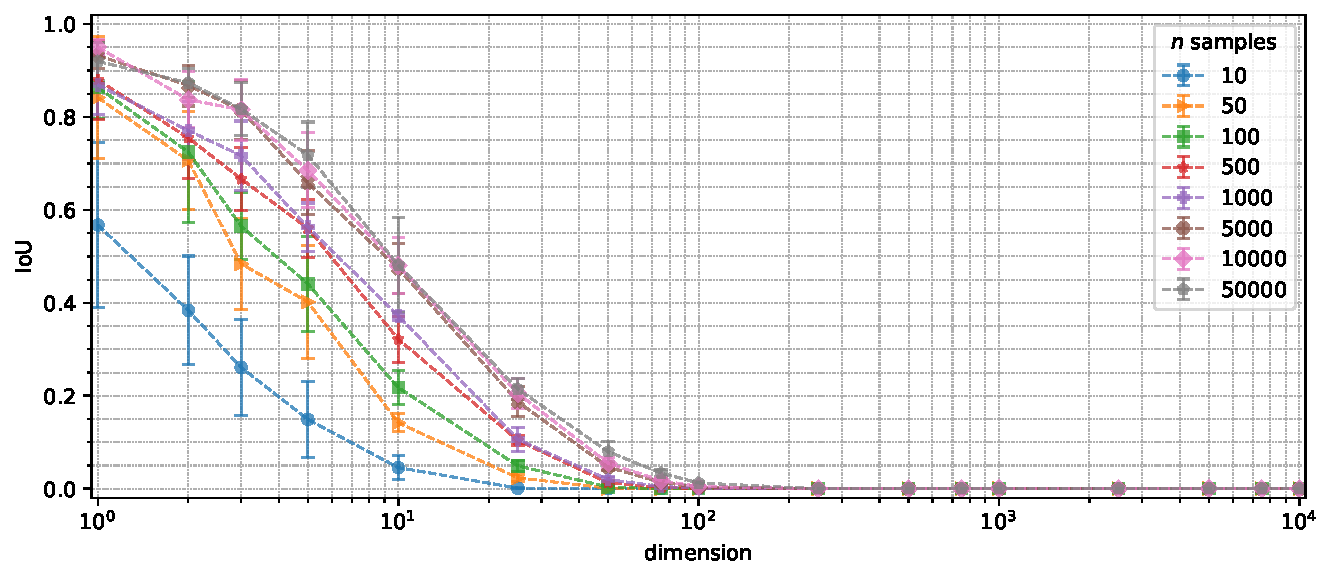
\includegraphics[width=\textwidth]{images/overlapping/trend-overlapping-IoU(dimension)-distribution_gaussian-samples_10,50,100,500,1000,5000,10000,50000-aggregated.pdf}
        \label{fig:iou-gaussian}
    \end{subfigure}

    \vspace{-0.75em}
    \begin{subfigure}[b]{0.9\textwidth}
        \centering
        \caption{\small Distribution $G = Triangular$}
        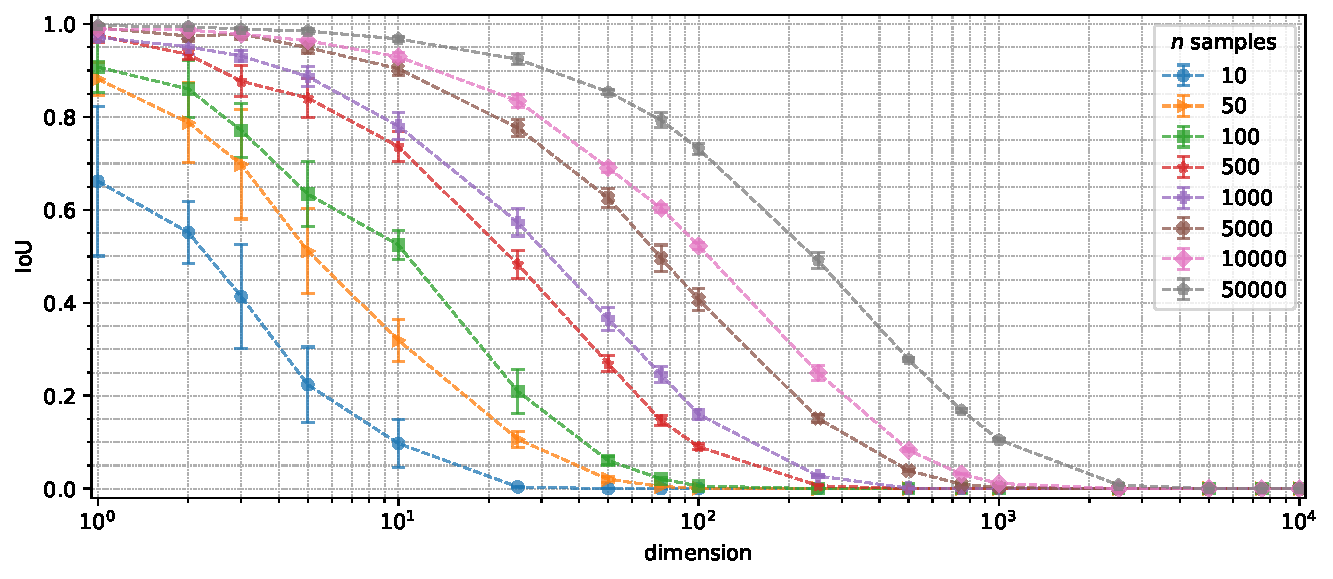
\includegraphics[width=\textwidth]{images/overlapping/trend-overlapping-IoU(dimension)-distribution_triangular-samples_10,50,100,500,1000,5000,10000,50000-aggregated.pdf}
        \label{fig:iou-triangular}
    \end{subfigure}

    \vspace{-0.75em}
    \begin{subfigure}[b]{0.9\textwidth}
        \centering
        \caption{\small Distribution $G = Uniform$}
        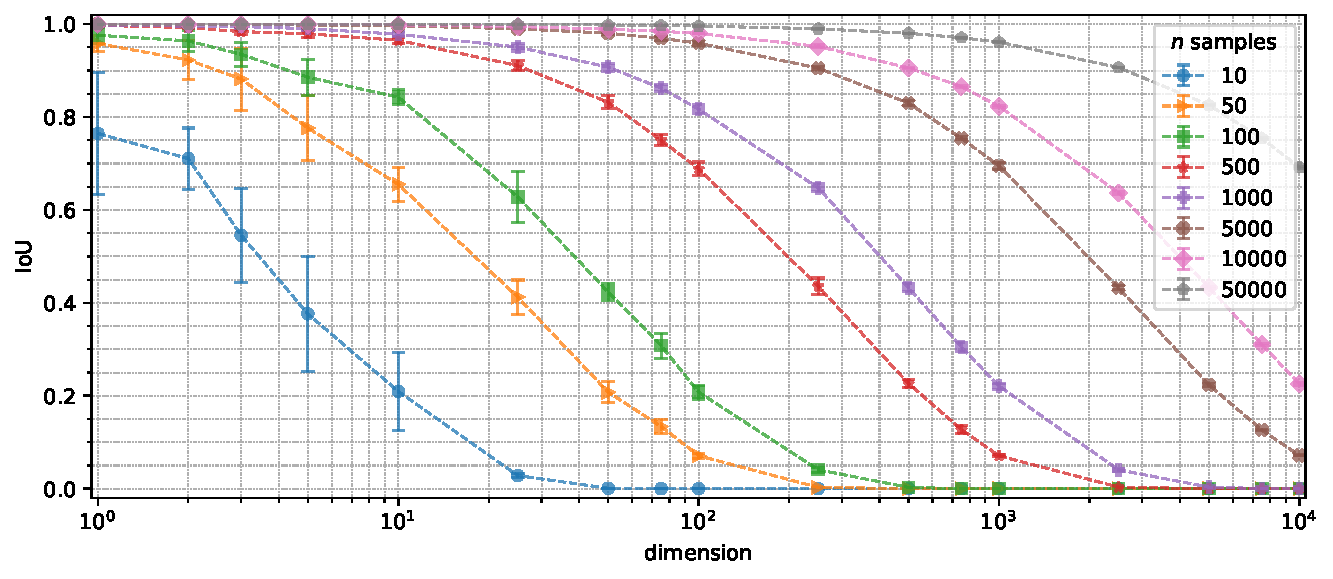
\includegraphics[width=\textwidth]{images/overlapping/trend-overlapping-IoU(dimension)-distribution_uniform-samples_10,50,100,500,1000,5000,10000,50000-aggregated.pdf}
        \label{fig:iou-uniform}
    \end{subfigure}

    \vspace{-0.5em}
    \caption{The relation between number of samples $n$ and dimension of feature space $d$ in the~task of recreating the same data cluster (represented as the bounding box). This task turns out significantly more difficult for $G = Gaussian$ distribution than for the distributions with finite output domain ($G = Triangular$, $G = Uniform$). The~results are aggregated for multiple generator seeds $\xi$ and displayed as averages with~error~bars~(standard deviation).}
    \label{fig:overlapping-1}
    \vspace{-3.2em}
\end{figure}

\begin{figure}[t]
    % StreamLit settings: width=9, height=4
    % X: [0.95, 10500.00]
    % Y: [-0.02, 1.02]
    \centering
    \vspace{-0.75em}
    \begin{subfigure}[b]{0.9\textwidth}
        \centering
        \caption{\small Distribution $G = Gaussian$ (detailed view)}
        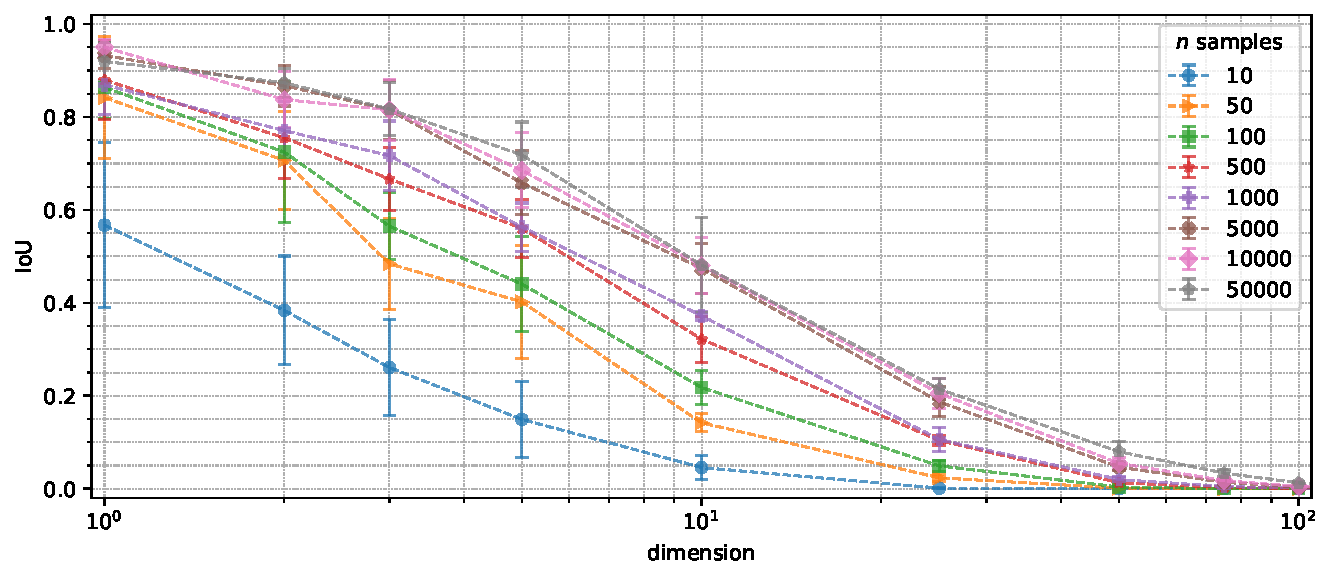
\includegraphics[width=\textwidth]{images/overlapping/trend-overlapping-IoU(dimension)-distribution_gaussian-samples_10,50,100,500,1000,5000,10000,50000-aggregated-detailed.pdf}
        \label{fig:iou-gaussian-detailed}
    \end{subfigure}

    \vspace{-0.75em}
    \begin{subfigure}[b]{0.9\textwidth}
        \centering
        \caption{\small Distribution $G = MVN$ ($g_{corr} = 0.5$, $f_{corr} = 0.5$)}
        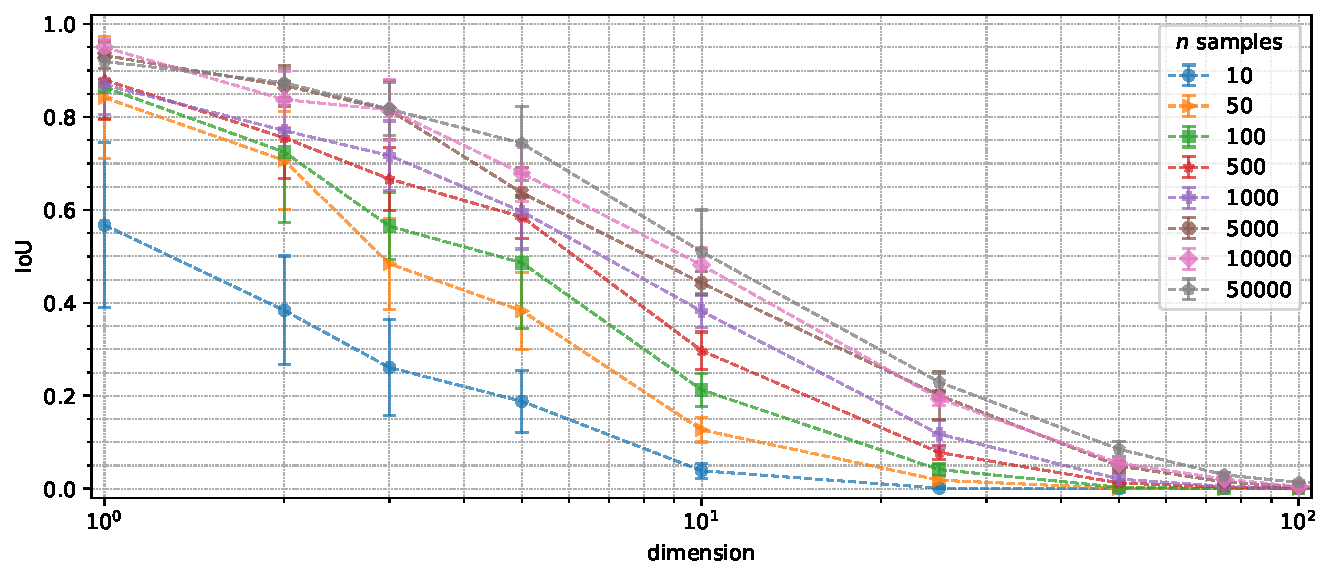
\includegraphics[width=\textwidth]{images/overlapping/trend-overlapping-IoU(dimension)-distribution_correlated-50-50-samples_10,50,100,500,1000,5000,10000,50000-aggregated-detailed.pdf}
        \label{fig:iou-correlated-detailed}
    \end{subfigure}

    \vspace{-0.75em}
    \begin{subfigure}[b]{0.9\textwidth}
        \centering
        \caption{\small Distribution $G = Gaussian$, utilizing Mahalanobis distance}
        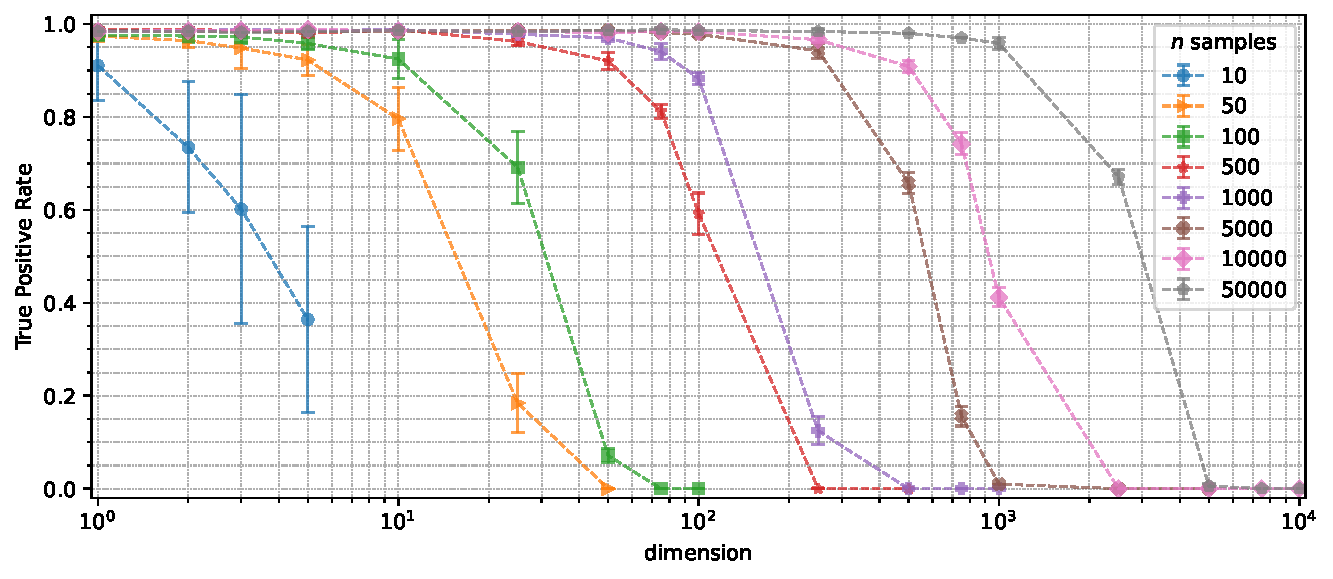
\includegraphics[width=\textwidth]{images/overlapping/trend-distributions-sens_99(dimension)-distance_8-distribution_gaussian-model_MD-samples_10,50,100,500,1000,5000,10000,50000-aggregated.pdf}
        \label{fig:tpr-gaussian-md}
    \end{subfigure}

    \vspace{-0.5em}
    \caption{The correlation of features, despite resulting in more concentrated clusters (smaller distances), is does not affect the results significantly (comparing subfigures \ref{fig:iou-gaussian-detailed} and \ref{fig:iou-correlated-detailed}). However, representing cluster with Mahalanobis distance model (i.e., hyperellipsoid-like structure), the overlapping can be effectively achieved ever for higher dimensions $d$. The~results are aggregated for multiple generator seeds $\xi$ and displayed as averages with~error~bars~(standard deviation).}
    \label{fig:overlapping-2}
    \vspace{-3.2em}
\end{figure}

\begin{figure}[t]
    % StreamLit settings: width=9, height=4
    % X: [0.95, 10500.00]
    % Y: [-0.02, 1.02]
    \centering
    \vspace{-0.75em}
    \begin{subfigure}[b]{0.9\textwidth}
        \centering
        \caption{\small Distribution $G = Gaussian$, utilizing k-Nearest Neighbors ($k=10$)}
        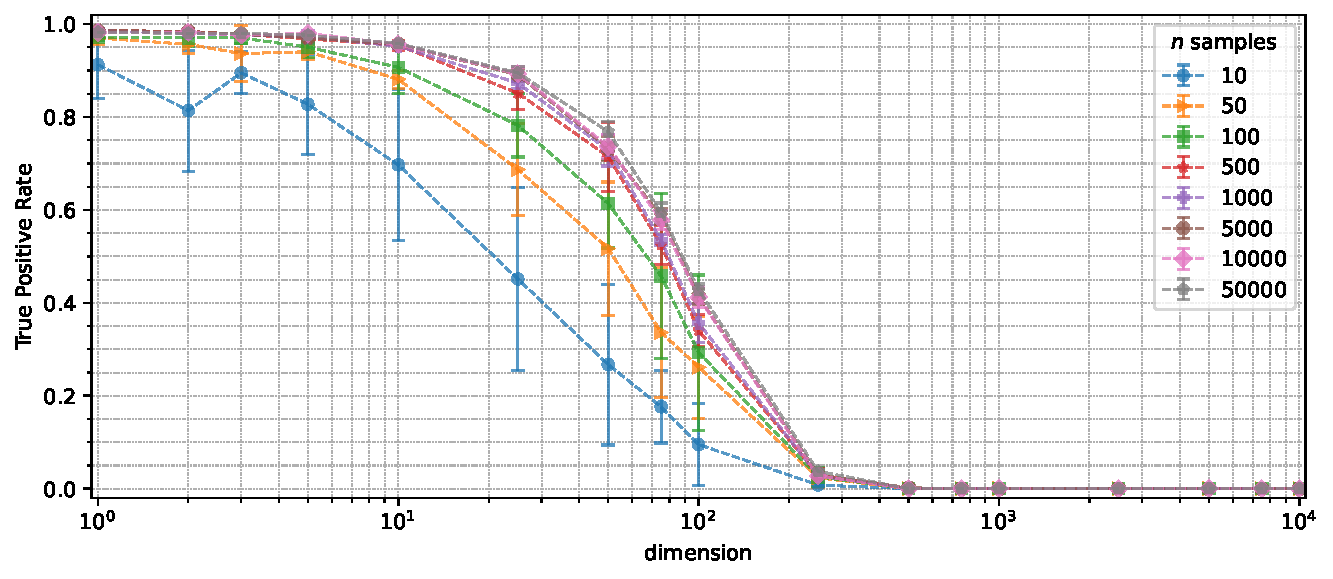
\includegraphics[width=\textwidth]{images/overlapping/trend-distributions-sens_99(dimension)-distance_1-distribution_gaussian-model_kNN-10-samples_10,50,100,500,1000,5000,10000,50000-aggregated.pdf}
        \label{fig:tpr-gaussian-knn}
    \end{subfigure}

    \vspace{-0.75em}
    \begin{subfigure}[b]{0.9\textwidth}
        \centering
        \caption{\small Distribution $G = Gaussian$, utilizing Local Outlier Factor ($k=10$)}
        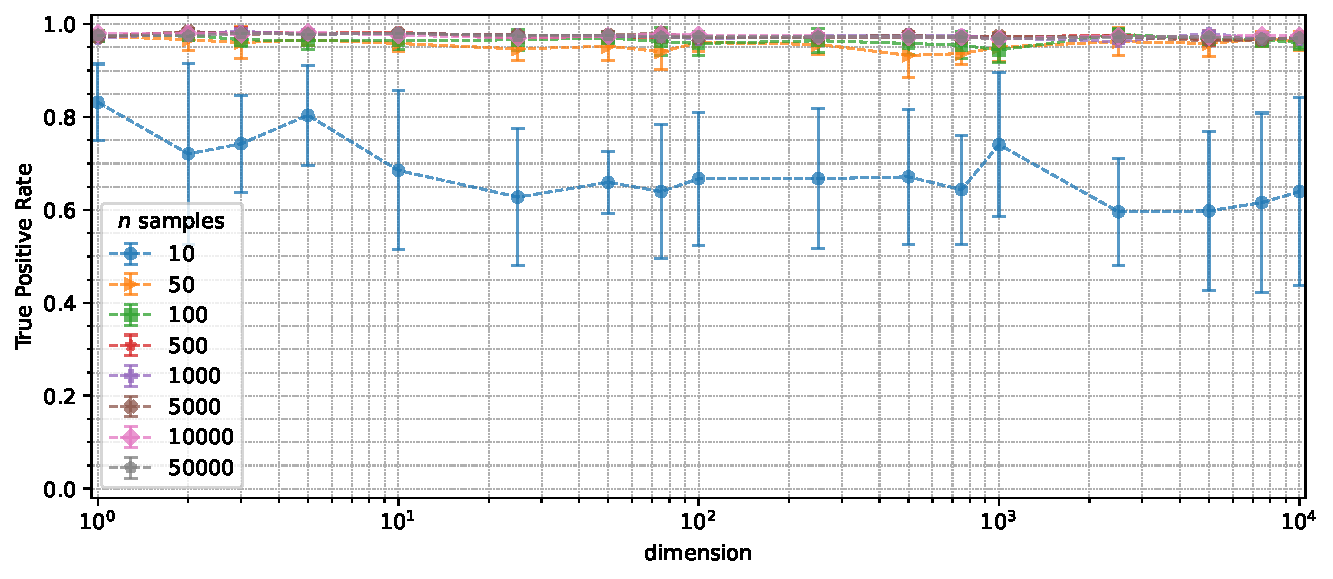
\includegraphics[width=\textwidth]{images/overlapping/trend-distributions-sens_99(dimension)-distance_1-distribution_gaussian-model_LOF-10-samples_10,50,100,500,1000,5000,10000,50000-aggregated.pdf}
        \label{fig:tpr-gaussian-lof}
    \end{subfigure}

    \vspace{-0.75em}
    \begin{subfigure}[b]{0.9\textwidth}
        \centering
        \caption{\small Distribution $G = Gaussian$, utilizing Standardized Euclidean distance}
        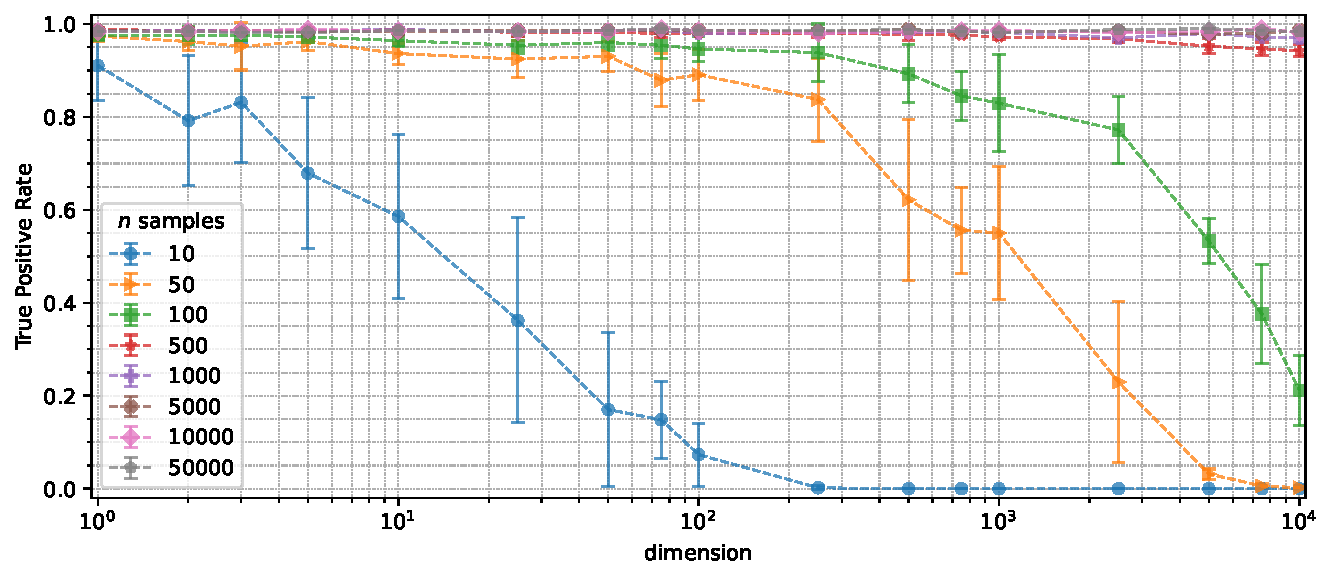
\includegraphics[width=\textwidth]{images/overlapping/trend-distributions-sens_99(dimension)-distance_1-distribution_gaussian-model_SED-samples_10,50,100,500,1000,5000,10000,50000-aggregated.pdf}
        \label{fig:tpr-gaussian-sed}
    \end{subfigure}

    \vspace{-0.5em}
    \caption{Clusters representations based on the distance measures described in~section \ref{section:measures} allow to obtain the effective overlapping ever for high features space dimensions $d$. For some methods the number of samples $n$ does not need to be high to~perform well; kNN's performance is related it selected parameter $k$ value. The~results are~aggregated for multiple generator seeds $\xi$ and displayed as averages with~error~bars~(standard deviation).}
    \label{fig:overlapping-3}
    \vspace{-3.2em}
\end{figure}

\cleardoublepage{}
